\documentclass[twoside,a4paper,12pt]{mwbk}

\usepackage[utf8]{inputenc}
%\usepackage{times}
\usepackage{amsmath,amssymb,amsthm}
\usepackage{xcolor}
\usepackage[final]{pdfpages}
\usepackage{graphicx}
%\usepackage[nottoc]{tocbibind}
\usepackage{caption}
\usepackage{subcaption}
\captionsetup{compatibility=false}
\usepackage{dsfont}
\usepackage{float}

\usepackage{booktabs}
\usepackage{array}

\renewcommand{\labelitemi}{$\bullet$}
\renewcommand{\labelitemii}{$\cdot$}
\renewcommand{\labelitemiii}{$\diamond$}
\renewcommand{\labelitemiv}{$\ast$}


\setlength{\parindent}{0pt}

%\usepackage{geometry}
%\newgeometry{tmargin=2.5cm, bmargin=2.5cm, lmargin=2.5cm, rmargin=2.5cm}

%\numberwithin{equation}{section}
%\numberwithin{figure}{section}
\renewcommand{\thefigure}{\thechapter.\arabic{figure}}

%\newcommand*{\doi}[1]{\href{http://dx.doi.org/#1}{doi: #1}}
%\newcommand*{\MR}[1]{\href{http://www.ams.org/mathscinet-getitem?mr=#1&return=pdf}{MR #1}}
%\newcommand*{\ZBL}[1]{\href{http://www.zentralblatt-math.org/zmath/en/advanced/?q=an:#1&format=complete}{Zbl #1}}


\newcommand{\1}[1]{\mathds{1}\left(#1\right)}

\newenvironment{diagrams}[2]{\begin{figure}[p]
	%\centering
	\begin{subfigure}{.5\textwidth}
		\centering
		\includegraphics[width=\textwidth]{wykresy/#1.png}
		\caption{}
		\label{#1}
	\end{subfigure}
	\begin{subfigure}{.5\textwidth}
		\centering
		\includegraphics[width=\textwidth]{wykresy/#2.png}
		\caption{}
		\label{#2}
	\end{subfigure}
	}
	{
	\end{figure}
	}

\newenvironment{subdiagrams}[2]{
		\begin{subfigure}{.5\textwidth}
			\centering
			\includegraphics[width=\textwidth]{wykresy/#1.png}
			\caption{}
			\label{#1}
		\end{subfigure}
		\begin{subfigure}{.5\textwidth}
			\centering
			\includegraphics[width=\textwidth]{wykresy/#2.png}
			\caption{}
			\label{#2}
		\end{subfigure}
	} {}

\newenvironment{subdiagram}[1]{
	\begin{subfigure}{\textwidth}
		\centering
		\includegraphics[width=.9\textwidth]{wykresy/#1.png}
		\caption{}
		\label{#1}
	\end{subfigure}
} {}

\theoremstyle{plain}
\newtheorem{thm}{Theorem}[chapter]

\theoremstyle{definition}
\newtheorem{defn}[thm]{Definition}


\begin{document}
	
\begin{titlepage}
	
\includepdf{title_page.pdf}
\end{titlepage}


\tableofcontents

\chapter*{Introduction}

\textit{ ** Few words about my thesis...
Generally what is a data mining, what are the wavelets, what are the applications in data mining and finally, what is the main purpose - edge detection. **}

Data mining is connected with computing huge amount of data, thus to analyse those data it is require to use algorithms with low computational complexity. Wavelet transform is very efficient.


\textit{ ** VERY GOOD PARAGRAPH - JUST NEEDS TO BE WRITE WITH DIFFERENT WORDS **}
	
\textit{ Real world data sets are usually not directly suitable for performing Data
Mining algorithms. They contain noise, missing values and may be inconsistent.
In addition, real world data sets tend to be too large and high-dimensional.
Wavelets provide a way to estimate the underlying function from the data. With
the vanishing moment property of wavelets, we know that only some wavelet
coefficients are significant in most cases. By retaining selective wavelet coefficients,
wavelet transform could then be applied to denoising and dimensionality
reduction. Moreover, since wavelet coefficients are generally decorrelated,
we could transform the original data into wavelet domain and then carry out
Data Mining tasks.}

Pre-processing:

Denoising signals and images. Wavelet denoising - transform data into wavelet domain, remove noise components (with lower frequency) and then back to the original domain.

Data Transformation?

Dimensionality reduction. The idea is to simplify data, by getting rid off the less relevant information. In a wavelet domain we retain only the largest coefficients. Then, after getting back to the original domain we obtain simplified data.

Machine learning processing:

Clustering. Low frequency parts are correlated with regions of objects concentration and the high frequency parts correspond to the areas with sudden changes in the objects distribution. Thus, clustering can be conducted by recognising correlated components in the wavelet domain.

Classification.
Regression.
Distributed Data Mining.
Similarity Search/Indexing.
Approximate Query Processing.
Traffic Modelling.

\chapter{Wavelets theory}
A ''wavelet'' literally means a small wave. This term says a lot about its nature. Wavelets are a family of functions which oscillates like wave and should be compactly supported. Additionally, the wavelet has zero mean.

\begin{defn}
Wavelets are created by scaling and shifting of the, so called, mother wavelet $\psi(t)$. The child wavelets are defined as

\begin{equation}
\label{eq:wavelets}
\psi^{(a,b)}(t)=|a|^{-\frac{1}{2}} \psi\left(\frac{t-b}{a}\right),\ a>0,
\end{equation}

where $a$ is a scale parameter and $b$ translation parameter.

\end{defn}

There are plenty of different mother wavelets, for example

\begin{figure}[h]
	\centering
	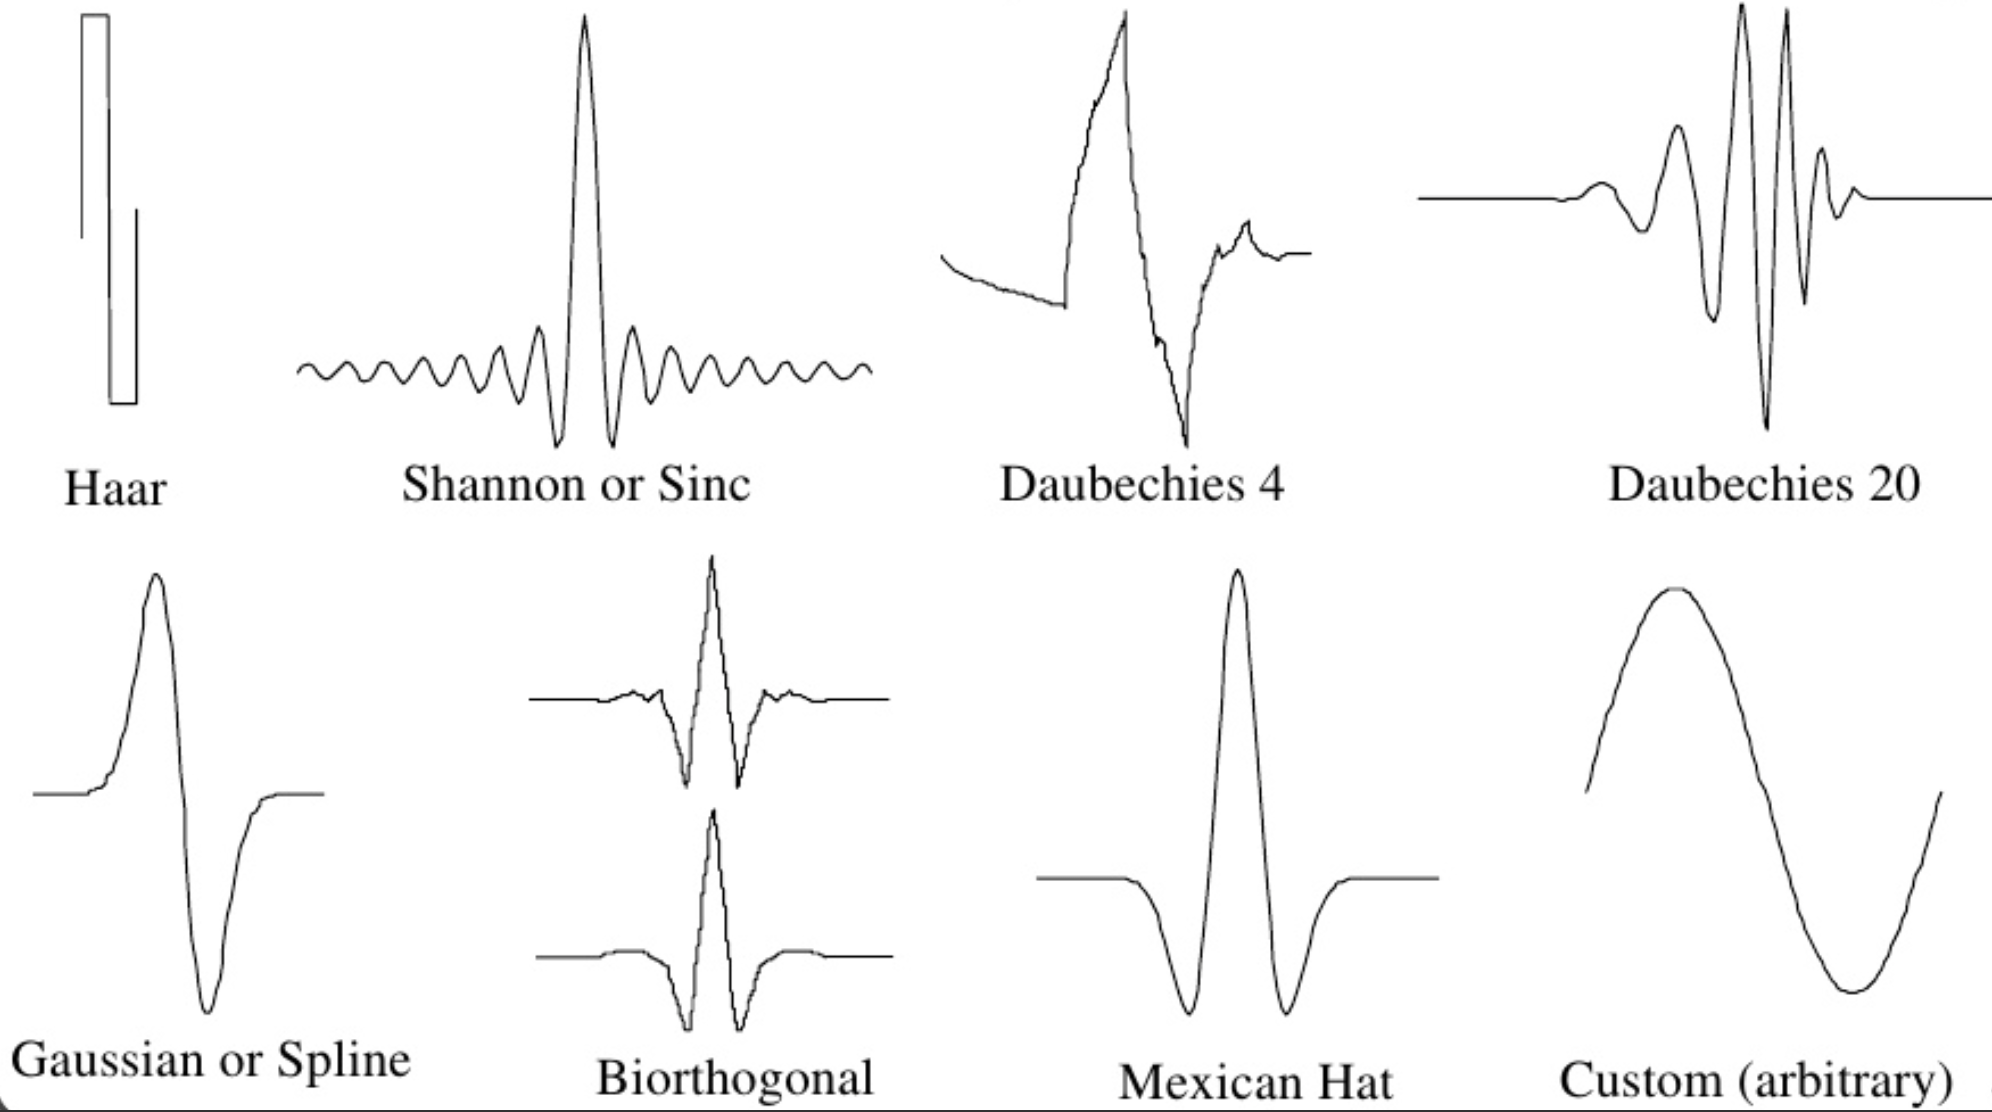
\includegraphics[width=\textwidth]{wavelets_with_bottom_line.png}
	\caption{Different types of wavelets.}
	\label{fig:wavelets}
\end{figure}

\textit{** Add more about wavelets properties! **}


\section{Daubechies wavelets}

Each type of wavelet function is more suitable for different applications. The best for image analysis are the Daubechies wavelets. 

\begin{defn}
Daubechies wavelets are collection of orthogonal and compactly supported functions. A denotation for those wavelets is $dbN$, where $N$ means a maximal number of vanishing moments.
\end{defn}

\begin{figure}[h]
	\centering
	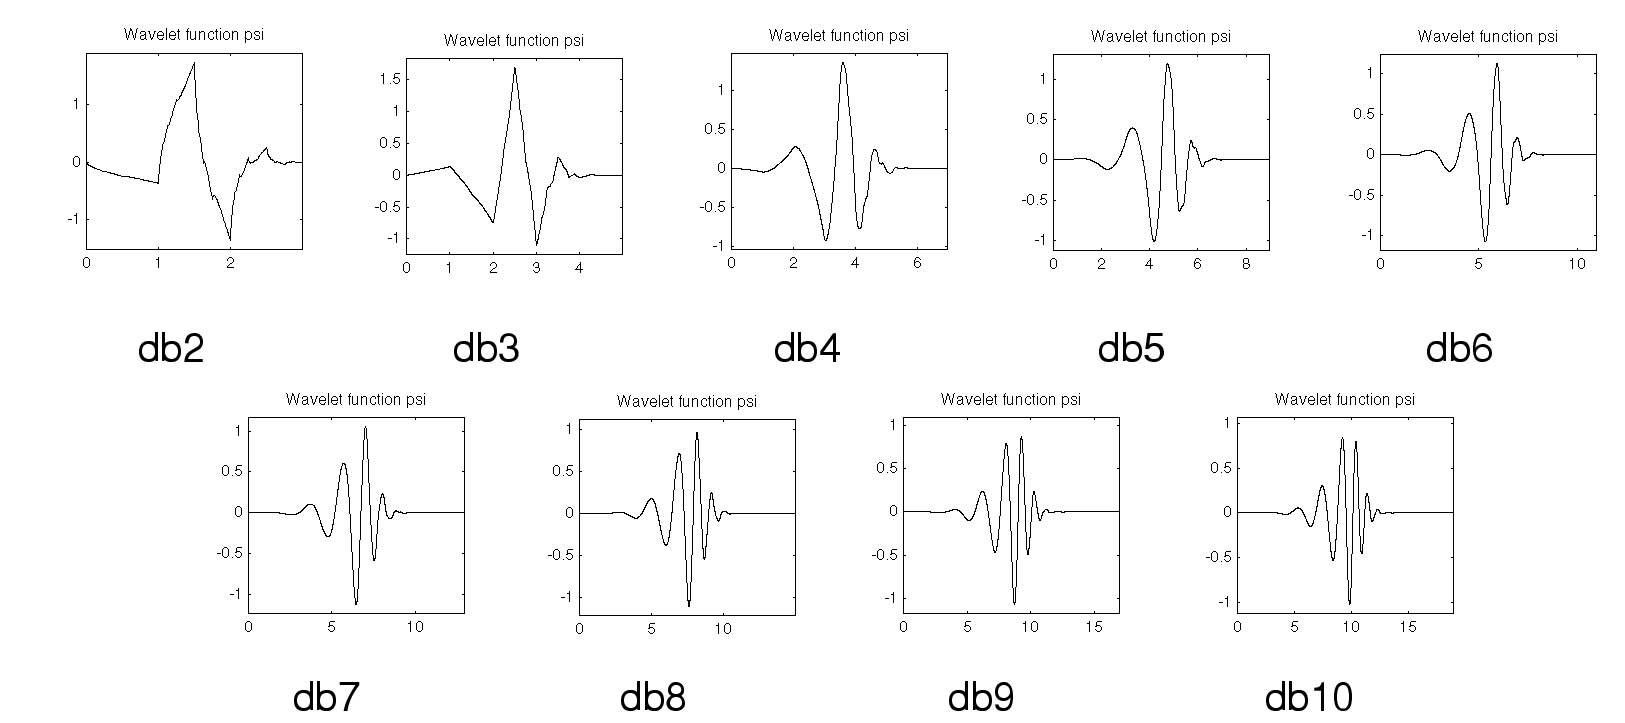
\includegraphics[width=\textwidth]{DB_N.png}
	\caption{Daubechies wavelets.}
	\label{fig:db_wavelets}
\end{figure}

\section{Wavelet Transform}

\textit{** Add some short introduction! -> po co to, co daje, do czego i dlaczego o tym piszemy  **}

\begin{defn}
Wavelet transform

\begin{equation}
W(a,b)=\int_{-\infty}^{\infty} y(t) a^{-\frac{1}{2}} \psi\left(\frac{t-b}{a}\right) dt,
\end{equation}

where $a$ is scale parameter, $b$ translation parameter and $y(t)$ original signal.
\end{defn}

\subsection{Wavelet transform vs Fourier transform}

\textit{** General information about integral transforms  **}

\begin{defn}
Fourier transform

\begin{equation}
Y(f)=\int_{-\infty}^{\infty} y(t) e^{-i\omega t} dt,
\end{equation}

where $y(t)$ is time domain signal and $Y(f)$ is frequency domain signal.
\end{defn}

\begin{table}[h]
\centering
\begin{tabular}{|p{0.5\linewidth}|p{0.5\linewidth}|}
\toprule
\textbf{ Wavelet transform} & \textbf{Fourier transform}
\\ \midrule
Suitable for stationary and non-\allowbreak -stationary signals 
& Suitable for stationary signals 
\\ \midrule
High time and frequency resolution
& Zero time resolution and very high frequency resolution     
\\ \midrule
Very suitable for studying the local behaviours of the signal
& No suitable  
\\ \midrule
Scaled and translated mother wavelets
& Sine and cosine waves
\\ \bottomrule
\end{tabular}
\caption{Differences between Wavelet Transform and Fourier Transform.}
\end{table}

What differs both transformations is the type of function. In Fourier case there are sine and cosine functions, wherein wavelet transform uses wavelets.

Why use the Wavelet transform?
Sine function oscillates on the whole real axis, thus it cannot represent abrupt changes. However, the Wavelet transform is localized in space and time, so it can be used to detect trends or sudden changes in signals and images. 

Moreover, wide range of wavelet functions is a main advantage of wavelet analysis.

\section{Discrete Wavelet transform}
There are two types of the wavelet transform:
\begin{itemize}
\item Continuous Wavelet Transform (CWT),
\item Discrete Wavelet Transform (DWT).
\end{itemize}

DWT is used to denoising and compression of signals and images. Also, DWT allows to detect smooth regions interrupted by edges or abrupt changes in contrast of images.

Scale and translation parameters are defined as

\begin{equation}
a = 2^j \text{ and } b = 2^j k,\ j,k=1,2,\ldots.
\end{equation}

to avoid redundancy in coefficients.


The figure \ref{fig:DWT} on a page \pageref{fig:DWT} shows how DWT works. Discrete Wavelet Transform splits signal with two filters: $g(n)$ - low pass filter (LPF) and $h(n)$ - high pass filter (HPF). The LPF captures a part with lower frequencies which refers to the main signal. Whereas, the HPF captures higher frequencies - a noise of the signal. Subsequently, both parts are downsampled by a factor of 2. This decomposition can be repeated on the LPF part of the signal. Hence, the next levels of DWT coefficients.

\begin{figure}[h]
	\centering
	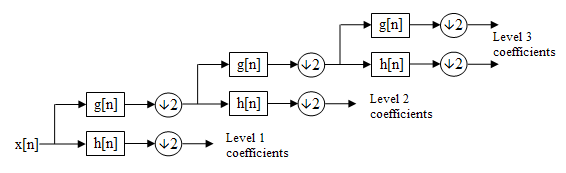
\includegraphics[width=\textwidth]{DWT.png}
	\caption{Discrete Wavelet transform on a signal $x(n)$.}
	\label{fig:DWT}
\end{figure}


\section{2-D Discrete Wavelet transform}
\label{sec:2D_DWT}

2-Dimensional Discrete Wavelet Transform works similar way as 1-D with High Pass Filter, Low Pass Filter and downsampling, except that one level of the decomposition includes double filtering, on columns and rows. The figure \ref{fig:2D_DWT} shows an image decomposition. Firstly, the DWT is applied on columns of the input image and then on the rows of the both outputs. Ultimately, there are four results:

\begin{itemize}
\item LL - result of LPF applied on both, columns and rows,
\item LH - result of LPF applied on columns and HPF on rows,
\item HL - result of HPF applied on columns and LPF on rows,
\item HH - result of HPF applied on both, columns and rows.
\end{itemize}  

\begin{figure}[h]
	\centering
	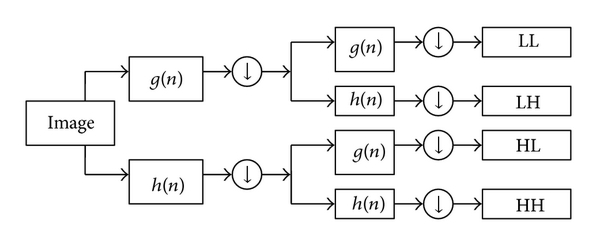
\includegraphics[width=\textwidth]{2D_DWT.JPG}
	\caption{2-D Discrete Wavelet transform on an image.}
	\label{fig:2D_DWT}
\end{figure}

Recall that the outcome of Low Pass Filter in the previous case was the main signal (without a noise). Thus, a 2-Dimensional equivalent is an approximation of an analysed image. The High Pass Filter captures high frequencies, then for an image the outcome are sudden changes in the image contrast. Now, lets focus on what exactly each result represent. First one, the LL is just an approximation of the initial image. Next, the LH shows abrupt changes in a horizontal direction, whereas the HL part presents similar issues but in a vertical direction. The HH shows sudden changes in a diagonal direction. In conclusion, the output of 2-D DWT gives us an approximation of the image and three parts with abrupt changes in different directions.

The Discrete Wavelet Transform has a wide range of applications in image processing, for example denoising, compressing 

\textit{** What are the possible applications of 2-D DWT - inne zastosowania w machine learning i data mining **}

What information gives us these sudden variations? Thanks to those we are able to find a places where two smooth regions meets. This kind of image anomaly could be interpreted as edges.

\section{Inverse Wavelet Transform}



\chapter{Edge detection} 
\label{ch:edge_detection}

In this chapter let us focus on the main goal of the thesis - edge detection. This problem is a special case of the data dimensionality reduction, which is a significant part of the pre-processing in data mining.

%An edge is a place where image brightness changes rapidly.

There are various methods to identify such discontinuities. The most popular are gradient based (e.g. Canny, Prewitt, Sobel) and Laplacian based. However, there is also another method, which provides similar results and can be more efficient in terms of computation. This method is based on the 2-Dimensional Discrete Wavelet Transform described in section \ref{sec:2D_DWT}. \newline

The mentioned method contains the following steps. \textit{** Link to article Edge detection **}
\begin{enumerate}
\item Convert image to grey scale.
\item Apply 2-D DWT on an image.
\item Remove the LL part.
\item Denoise the LH, HL and HH coefficients.
\item Reconstruct the initial image.
\item Post-processing - modify contrast to emphasize obtained edges.
\end{enumerate}

\section{Implementation of an algorithm}
\label{sec:implementation}

The algorithm is implemented in \texttt{Python} using \texttt{PyWavelets} package. There are used also auxiliary packages like: \texttt{numpy}, \texttt{matplotlib}, \texttt{PIL} and \texttt{scipy}. The \texttt{PyWavelets} package contains all features required to edge detection algorithm, i.e. 2D Forward and Inverse Discrete Wavelet Transform, build-in many wavelet functions and thresholding functionality (used to denoise coefficients).

Lets go deeper into algorithm, using a simple example - white square on a black background.

\begin{figure}[h]
	\centering
	
\includegraphics[width=0.3\textwidth]{graphs/square.png}
	\caption{An initial image - a white square.}
\end{figure}

Initially, a colour image must be simplified by conversion to grey scale. Edges are recognised as changes in brightness, so a single pixel should contains only information about a colour (black) intensity. Our initial image is already black and white so we do not need to convert it. Now, we can apply the 2D DWT function. As a result, according to the description in section \ref{sec:2D_DWT}, we obtain four components of wavelet coefficients: LL, LH, HL and HH shown on a graph \ref{fig:square_coeffs}. It is clearly visible that the LL part reflects the initial image and the rest components contains information about rapid brightness changes in particular directions. 

\begin{figure}[h]
	\centering
	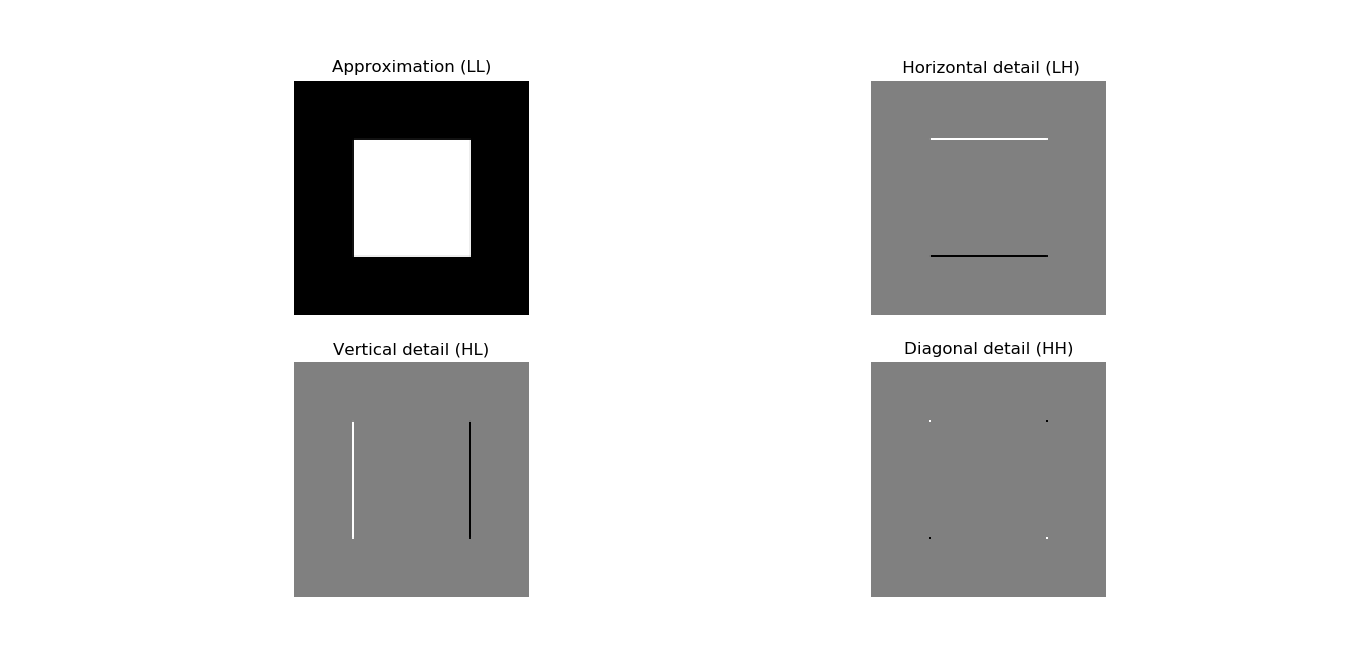
\includegraphics[width=\textwidth]{graphs/square_db2_coeffs.png}
	\caption{2-D DWT coefficients.}
	\label{fig:square_coeffs}
\end{figure}

Thus, we are interested only in components which gives information about edges, so we remove the approximation part - figure \ref{fig:square_coeffs_d}.

\begin{figure}[h]
	\centering
	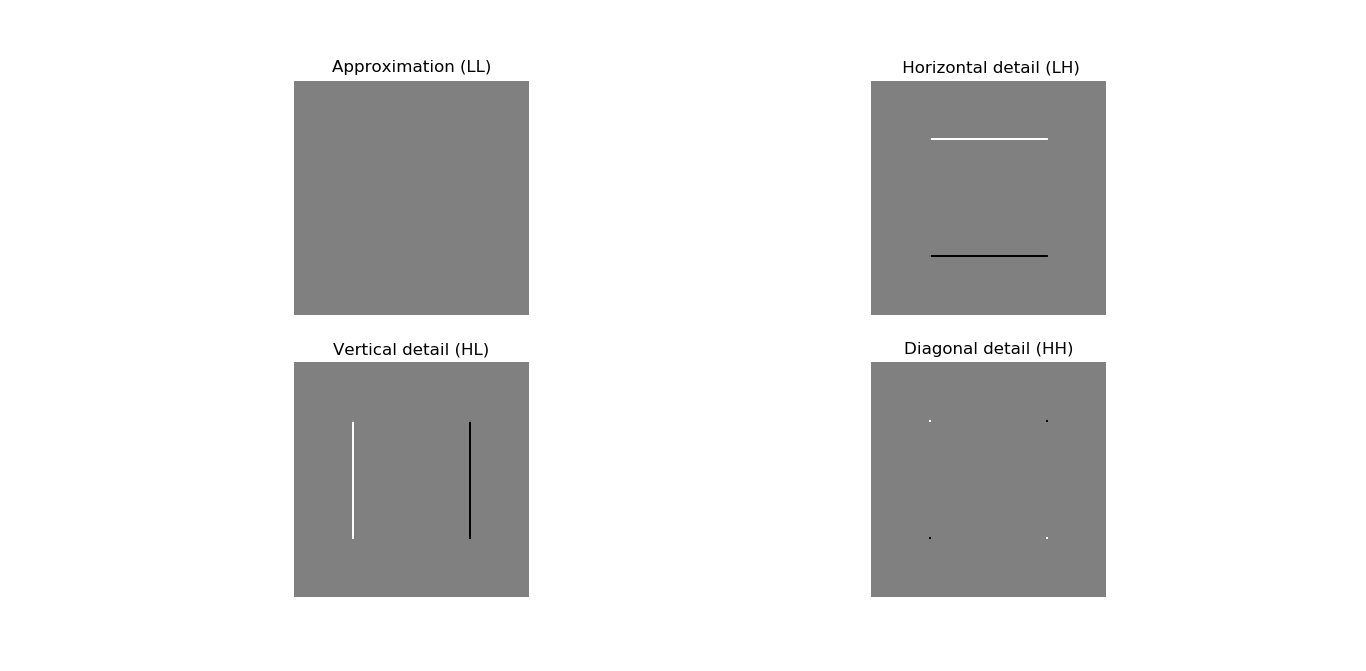
\includegraphics[width=\textwidth]{graphs/square_db2_coeffs_d.png}
	\caption{2-D DWT coefficients with removed the LL part.}
	\label{fig:square_coeffs_d}
\end{figure}

Subsequently, remaining components can be denoised. It means, we can get rid off small, insignificant coefficients by thresholding. More about setting the threshold is described in section \ref{sec:threshold}. This simple example do not require any denoising, so lets go further.

The last main step is reconstruction of the initial image, i.e. application an inverse DWT on the denoised coefficients. In the result, we obtain edges of the initial image presented on a graph \ref{fig:square_idwt}.

\begin{figure}[h]
	\centering
	
\includegraphics[width=0.3\textwidth]{graphs/square_db2.png}
	\caption{A reconstructed image showing the edges.}
	\label{fig:square_idwt}
\end{figure}

At the end, we can manipulate contrast to emphasize obtained lines. Currently, a background has grey colour and the edges are white or black. Therefore, using simple mathematical calculations we can modify image to have black background and white edges. It is enough to get an absolute value, subtract 128 and then scale by multiplying 2 times.

\textit{** Calculations taken from article Edge detection. Add note about values in an image array **}

Finally, we obtain the edges of the square shown on the figure \ref{fig:square_idwt_pp}.

\begin{figure}[h]
	\centering
	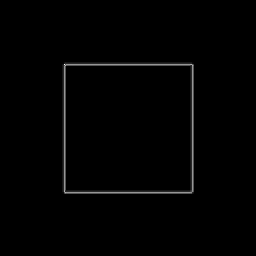
\includegraphics[width=0.3\textwidth]{graphs/square_db2_pp.png}
	\caption{The edges of the square image after post-processing.}
	\label{fig:square_idwt_pp}
\end{figure}

\section{Thresholding}
\label{sec:threshold}

The wavelets property of vanishing moments guarantee that bigger wavelet coefficients are more significant. Thus, the noise is placed in lowest values. To remove those values we can use, so-called, thresholding, which has two types: hard and soft. Lets denote $\lambda$ as threshold value and $d$ as wavelet coefficient. The hard thresholding is defined as follow

\begin{equation}
D^H(d|\lambda)=
\begin{cases}
0, & \text{for } |d| \leq \lambda, \\
d, & \text{for } |d| > \lambda.
\end{cases}
\end{equation}

It assigns zero value for coefficients below the set threshold. The soft thresholding works in the same way on the coefficients smaller than $\lambda$, but additionally the coefficient bigger than the set threshold are ''shrinked'' towards zero, as it is defined below.

\begin{equation}
D^S(d|\lambda)=
\begin{cases}
	0, & \text{for } |d| \leq \lambda, \\
	d-\lambda, & \text{for } d > \lambda, \\
	d+\lambda, & \text{for } d < -\lambda.
\end{cases}
\end{equation}


\subsection{Hard or soft thresholding}

To see the differences between both types of thresholding lets consider a noisy image (fig. \ref{fig:square_s10}).

\begin{figure}[h]
	\centering
	
\includegraphics[width=0.3\textwidth]{graphs/square_s10.png}
	\caption{A noisy square image.}
	\label{fig:square_s10}
\end{figure}

The coefficients of 2-D DWT are shown on the graph \ref{fig:square_s10_coeffs}.

\begin{figure}[h]
	\centering
	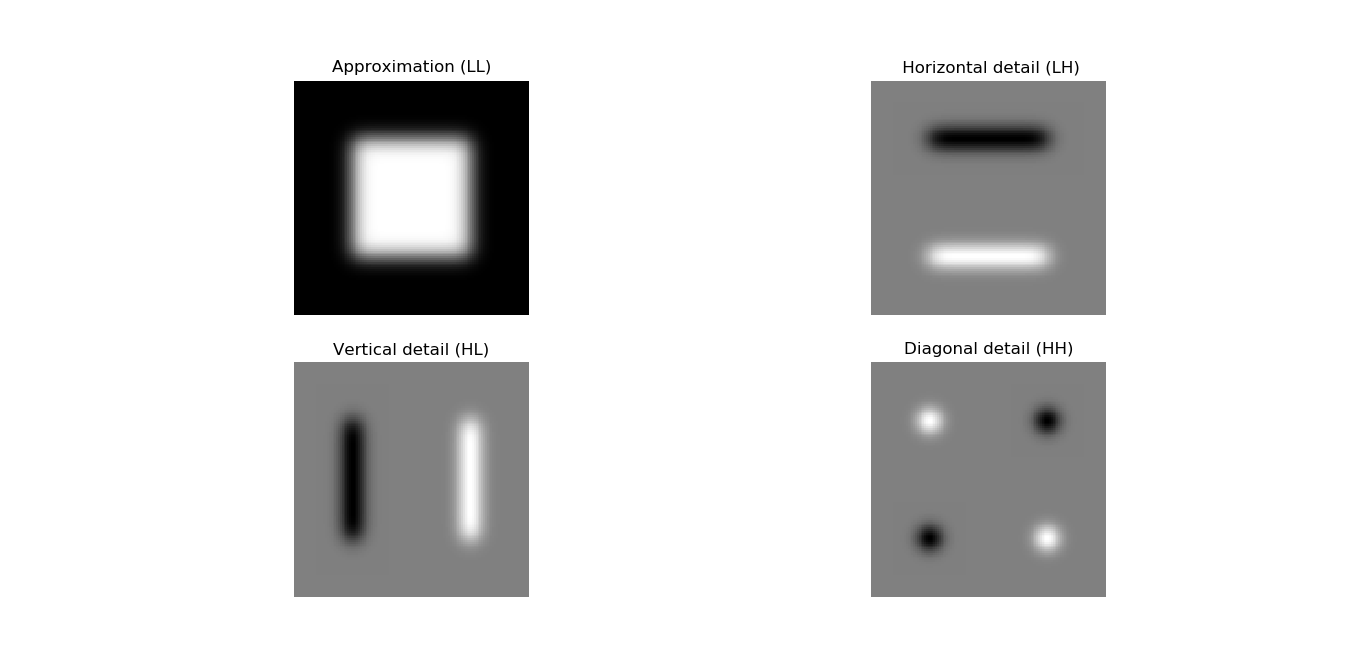
\includegraphics[width=\textwidth]{graphs/square_s10_db1_coeffs.png}
	\caption{2-D DWT coefficients.}
	\label{fig:square_s10_coeffs}
\end{figure}

Now, according to the edge detection algorithm, we remove the LL component and we can denoise the other ones. Results of hard and soft thresholding are presented respectively on a figures \ref{fig:square_s10_hard_coeffs_d} and \ref{fig:square_s10_soft_coeffs_d}.

\begin{figure}[h]
	\centering
	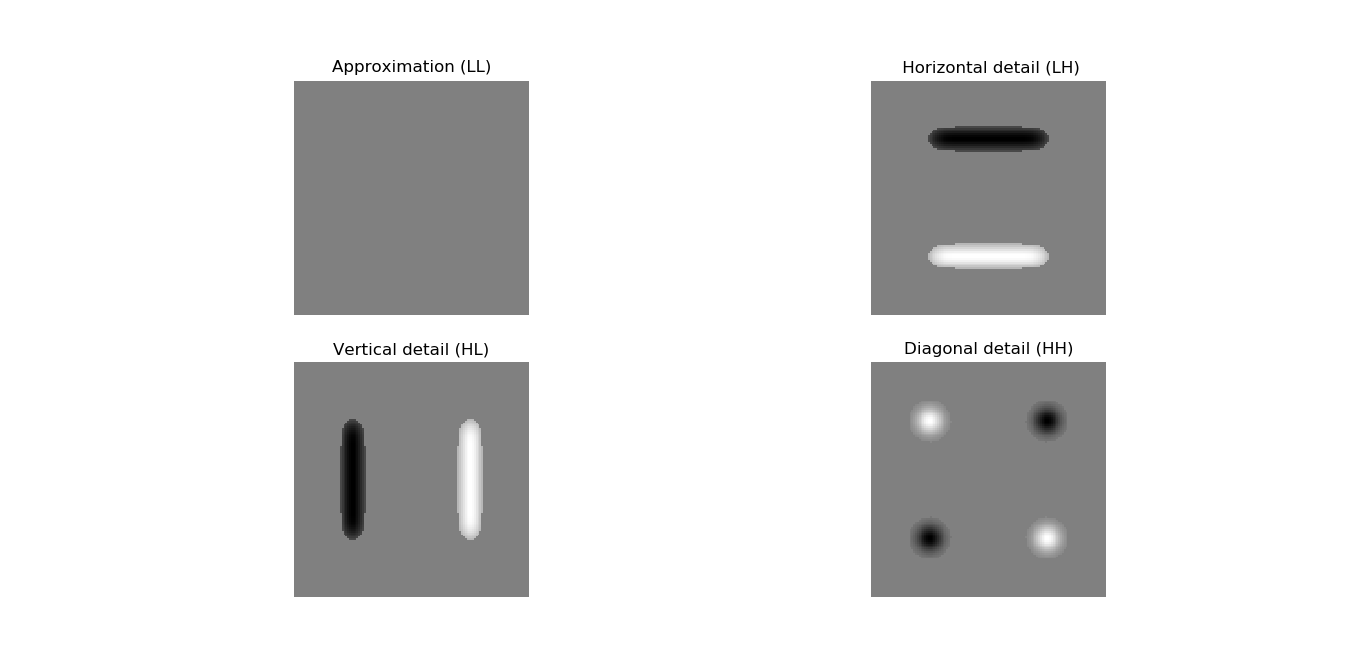
\includegraphics[width=\textwidth]{graphs/square_s10_db1_hard_coeffs_d.png}
	\caption{2-D DWT coefficients after hard thresholding.}
	\label{fig:square_s10_hard_coeffs_d}
\end{figure}

\begin{figure}[h]
	\centering
	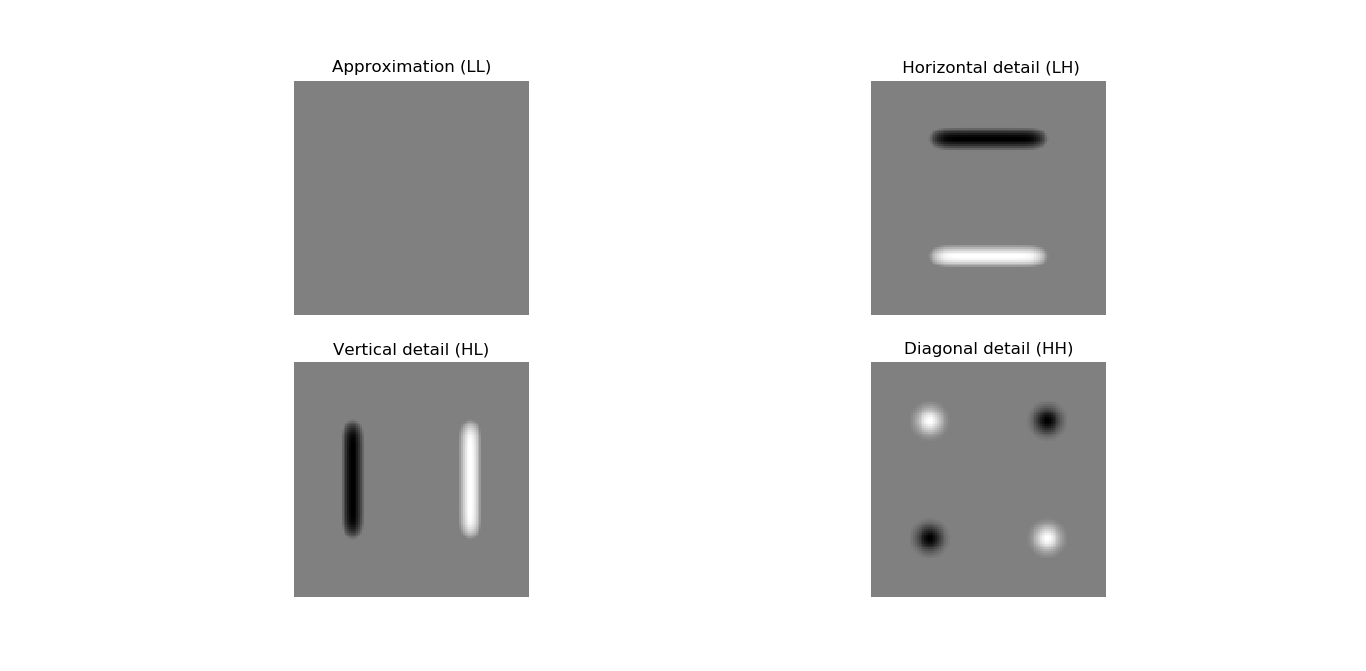
\includegraphics[width=\textwidth]{graphs/square_s10_db1_soft_coeffs_d.png}
	\caption{2-D DWT coefficients after soft thresholding.}
	\label{fig:square_s10_soft_coeffs_d}
\end{figure}

We can see the distinction between both thresholding, especially on the LH and HL components. After soft one the lines are smoother and slightly narrower, then in the other case. Therefore, the soft thresholding seems to be better for edge detection. Because of the smoother results, it is especially useful for the real life images, where edges are often blurred. To confirm this conclusion lets compare the final results, after inverse DWT (fig. \ref{fig:square_s10_idwt_pp})

\begin{figure}[h]
	\begin{subdiagrams2}{square_s10_db1_hard_pp}{hard}{square_s10_db1_soft_pp}{soft}
	\end{subdiagrams2}
	\centering
	\caption{Results of edge detection with hard and soft thresholding.}
	\label{fig:square_s10_idwt_pp}
\end{figure}

%\newpage

\subsection{Setting the threshold}
The corollary from the previous subsection is that the soft thresholding provides better results for edge detection. However, there is also a question how to choose the value of a threshold $\lambda$ to denoise coefficients and do not loose any significant information. A simple idea is to get a quantile of the coefficients in the specific components.

We decided to start with a quantile on level 0.95. It occurs to be accurate for the majority of standard images. All the earlier results are computed for threshold set as 0.95 quantile. Although, images which are noisier could require changing the quantile level.

Lets consider three images of basic diamond shape with different noisiness $\sigma$, shown on the figure \ref{fig:diamonds}.

\begin{figure}[h]
	\begin{subdiagrams3}{diamond_s16}{$\sigma=16$}{diamond_s10}{$\sigma=10$}{diamond_s4}{$\sigma=4$}
	\end{subdiagrams3}
	\centering
	\caption{The initial images of diamond with different noise level.}
	\label{fig:diamonds}
\end{figure}

At first, see how looks the result with mentioned earlier threshold set as 0.95 quantile (fig. \ref{fig:diamonds_95}). Algorithm found the edges properly but they are quite wide, especially for the noisier image. Lets try to increase the threshold to quantile on the 0.99 level. The results are presented on the graph \ref{fig:diamonds_99}. It can be seen that for (b) and (c) images the edges are narrower and visible. Nevertheless, result for the (a) image is incorrect, threshold is too high and too much information is removed.

\begin{figure}[h]
	\begin{subdiagrams3}{diamond_s16_db1_95_pp}{$\sigma=16$}{diamond_s10_db1_95_pp}{$\sigma=10$}{diamond_s4_db1_95_pp}{$\sigma=4$}
	\end{subdiagrams3}
	\centering
	\caption{The recognized edges for the diamonds with $\lambda$ equals 0.95 quantile.}
	\label{fig:diamonds_95}
\end{figure}

\begin{figure}[h]
	\begin{subdiagrams3}{diamond_s16_db1_99_pp}{$\sigma=16$}{diamond_s10_db1_99_pp}{$\sigma=10$}{diamond_s4_db1_99_pp}{$\sigma=4$}
	\end{subdiagrams3}
	\centering
	\caption{The recognized edges for the diamonds with $\lambda$ equals 0.99 quantile.}
	\label{fig:diamonds_99}
\end{figure}

Hence, lets consider one more threshold on a 0.98 quantile level. The recognised edges for (a) and (b) images are presented on the figure \ref{fig:diamonds_98}. For this threshold edges are correctly detected.

\begin{figure}[h]
	\begin{subdiagrams3}{diamond_s16_db1_98_pp}{$\sigma=16$}{diamond_s10_db1_98_pp}{$\sigma=10$}{diamond_s4_db1_98_pp}{$\sigma=4$}
	\end{subdiagrams3}
	\centering
	\caption{The recognized edges for the diamonds with $\lambda$ equals 0.98 quantile.}
	\label{fig:diamonds_98}
\end{figure}


In conclusion, for noisier images increasing the threshold provides more accurate result, but it must be done carefully to not ignore crucial informations. Additionally, when image shows one sharp object and noisy background, by increasing the threshold we can control the amount of background details in the result.

\section{Selection of a wavelet type}

As it was mentioned in the chapter \ref{ch:theory}, the family of Daubechies wavelets are very suitable to image processing. Therefore, we carry out the edge detection using this kind of wavelets. However, each of $dbn$ wavelet has slightly different properties, mainly because of changing the $n$ value, the number of vanishing moments.

Lets consider which of the Daubechies wavelets, are the best for edge detection problem. Remark that, all of the analysis below are conducted with the soft threshold set as 95 quantile. The figure \ref{fig:camera_haar} (a) presents an example image in grey scale, the man with a camera.
Firstly, we take the simplest one, Haar ($db1$) wavelet. Looking at the detected edges on the figure \ref{fig:camera_haar} (b), we can clearly observe boundaries of main objects - the man and a camera. Not every edge is recognised, e.g. a hand of the man, because of a small difference in brightness.

\begin{figure}[h]
	\centering
	\begin{mainsubdiagrams2}{camera}{original}{camera_haar_pp}{$db1$}
	\end{mainsubdiagrams2}
	
	\caption{A man with a camera and detected edges using Haar wavelet.}
	\label{fig:camera_haar}
\end{figure}

Next, lets consider Daubechies wavelets with the higher $n$. The results for selected $n$ are presented on the figure \ref{fig:camera_daubechies}. They provide worse edge approximation than the Haar transform. There are small differences between specific $dbn$ but no regularity can be seen.

\begin{figure}[h]
	\centering
	\begin{mainsubdiagrams2}{camera_db2_pp}{$db2$}{camera_db4_pp}{$db4$}
	\end{mainsubdiagrams2}
	
	\begin{mainsubdiagrams2}{camera_db6_pp}{$db6$}{camera_db8_pp}{$db8$}
	\end{mainsubdiagrams2}
	
	\caption{A man with a camera - detected edges using selected Daubechies wavelets.}
	\label{fig:camera_daubechies}
\end{figure}

Based on the example above, the conclusion can be made that the Haar wavelet provides the best results in edge detection. Unfortunately, this simplest wavelet not always works properly. For the basic square image, the Haar transform does not recognise any edges (fig. \ref{fig:square_daubechies} (b)). Hence, we need to apply Daubechies wavelet with the bigger $n$ value. For the $n=2$ or more, the square's perimeter is correctly detected and the results for different $n=2,3,\ldots$ are very similar to each other (fig. \ref{fig:square_daubechies}). The whole edge detection analysis presented in section \ref{sec:implementation} was made with $db2$ wavelets.

\begin{figure}[h]
	\centering
	\begin{subdiagrams2}{square}{original}{square_haar_pp}{$db1$}
	\end{subdiagrams2}
	
	\begin{subdiagrams2}{square_db2_pp}{$db2$}{square_db4_pp}{$db4$}
	\end{subdiagrams2}
	
	\caption{A simple square - detected edges using selected Daubechies wavelets.}
	\label{fig:square_daubechies}
\end{figure}

Lets consider the third example, a noisy square (fig. \ref{fig:rotated_square_daubechies}). In this case only the $db1$ (Haar) provides proper result - the square's perimeter. The edge is quite wide, but this feature can be improved by thresholding described in section \ref{sec:threshold}. The rest of presented results (c) - (f) are incorrect. Therefore, we revealed that the Haar wavelet is also the most appropriate for recognizing edges on noisy images. 

\begin{figure}[h]
	\centering
	\begin{subdiagrams2}{rotated_square}{original}{rotated_square_haar_pp}{$db1$}
	\end{subdiagrams2}

	\begin{subdiagrams2}{rotated_square_db2_pp}{$db2$}{rotated_square_db4_pp}{$db4$}
	\end{subdiagrams2}
	
	\begin{subdiagrams2}{rotated_square_db6_pp}{$db6$}{rotated_square_db8_pp}{$db8$}
	\end{subdiagrams2}
	
	\caption{A noisy rotated square - detected edges using selected Daubechies wavelets.}
	\label{fig:rotated_square_daubechies}
\end{figure}

The last example is a photo of a frog presented on the figure \ref{fig:frog_daubechies}. Incidentally, this photo was made in The Wroclaw Botanical Garden. Back to the results, it can be seen that for Haar wavelet (b) edges are the clearest and sharpest. On the other graphs, (c) and (d), the contour of the frog is also visible, but it is more blurred. Moreover, the bigger $n$, the edges are more unclear.

\begin{figure}[h]
	\centering
	\begin{subdiagram}{frog}{original}
	\end{subdiagram}

	\begin{subdiagram}{frog_haar_pp}{$db1$}
	\end{subdiagram}
	
	\begin{subdiagram}{frog_db2_pp}{$db2$}
	\end{subdiagram}

	\begin{subdiagram}{frog_db6_pp}{$db6$}
	\end{subdiagram}
	
	\caption{A frog - detected edges using selected Daubechies wavelets.}
	\label{fig:frog_daubechies}
\end{figure}

To sum up, for the majority of images the Haar wavelet provides the best results. However, there are cases, when the $db1$ wavelet fails. Then, it is required to use another of Daubechies wavelet, e.g. $db2$.


\chapter{}

\textit{** Results **}

\listoffigures
\listoftables

%\bibliographystyle{unsrt} % w kolejności pojawienia
\bibliographystyle{abbrv} % w kolejności alfabetycznej
\bibliography{bibliography_KK}
\nocite{WaveletMethodsInDataMining}
\nocite{DataManing}
\nocite{WaveletSupportVectorMachine}
\nocite{WaveletNotes}
\nocite{EdgeDetection}
\nocite{BiomedicalImages}

	
\end{document}